% Fonte da Figura 3 (recriado em TikZ a partir do PNG original mheg_componentes.png;
% unica mudanca de conteudo: a linha de supressao da caixa verde agora diz
% "otherwise reuse the emitted probability: p_t <- p_{t-1}" — a propagacao de h
% foi removida, em conformidade com o Algoritmo 1/§3.4 (semantica avaliada:
% janela W=96 recomputada; estado reinicializado a cada atualizacao).
\documentclass[tikz,border=6pt]{standalone}
\usetikzlibrary{positioning,arrows.meta,calc}
\begin{document}
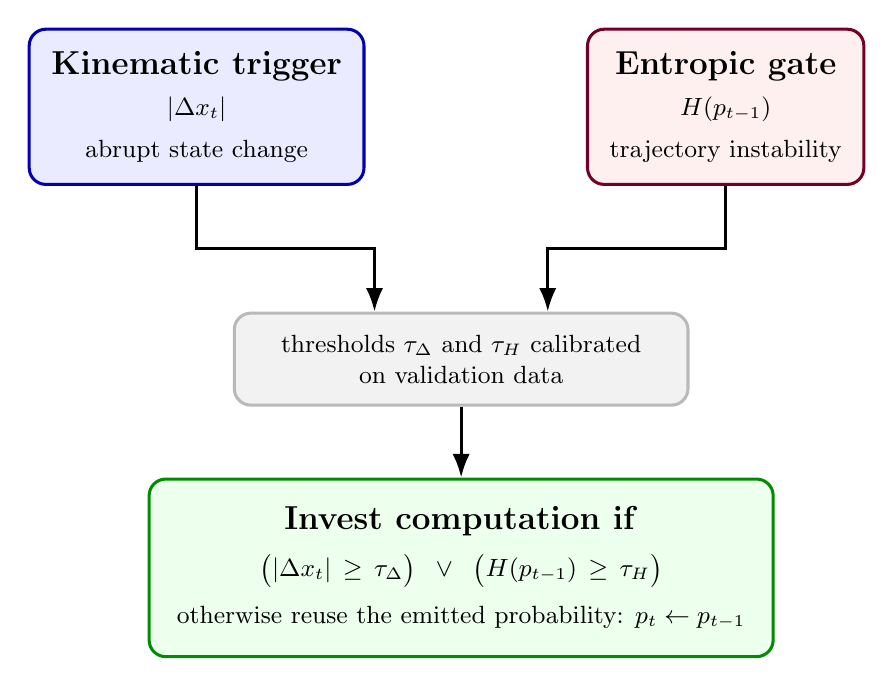
\begin{tikzpicture}[
  font=\small,
  box/.style={rounded corners=6pt, line width=1.1pt, align=center, inner sep=8pt},
  arr/.style={-{Latex[length=3mm,width=2.2mm]}, line width=1.1pt}
]
\node[box, draw=blue!70!black, fill=blue!8] (kin)
  {\textbf{\large Kinematic trigger}\\[4pt] $|\Delta x_t|$\\[4pt] abrupt state change};
\node[box, draw=purple!60!black, fill=red!6, right=28mm of kin] (ent)
  {\textbf{\large Entropic gate}\\[4pt] $H(p_{t-1})$\\[4pt] trajectory instability};
\coordinate (mid) at ($(kin.south)!0.5!(ent.south)$);
\node[box, draw=gray!55, fill=gray!10, text width=52mm] (thr) at ($(mid)+(0,-22mm)$)
  {thresholds $\tau_\Delta$ and $\tau_H$ calibrated\\on validation data};
\node[box, draw=green!55!black, fill=green!7, below=9mm of thr, inner sep=10pt] (dec)
  {\textbf{\large Invest computation if}\\[6pt]
   $\bigl(|\Delta x_t| \,\ge\, \tau_\Delta\bigr) \;\;\lor\;\; \bigl(H(p_{t-1}) \,\ge\, \tau_H\bigr)$\\[6pt]
   otherwise reuse the emitted probability: $p_t \leftarrow p_{t-1}$};
\draw[arr] (kin.south) -- ++(0,-8mm) -| ([xshift=-11mm]thr.north);
\draw[arr] (ent.south) -- ++(0,-8mm) -| ([xshift=11mm]thr.north);
\draw[arr] (thr.south) -- (dec.north);
\end{tikzpicture}
\end{document}
